\section{Example \Filestores{}}
\label{sec:examples}


\begin{figure}
\vskip -.25in
\hskip -.15in \scalebox{.30}{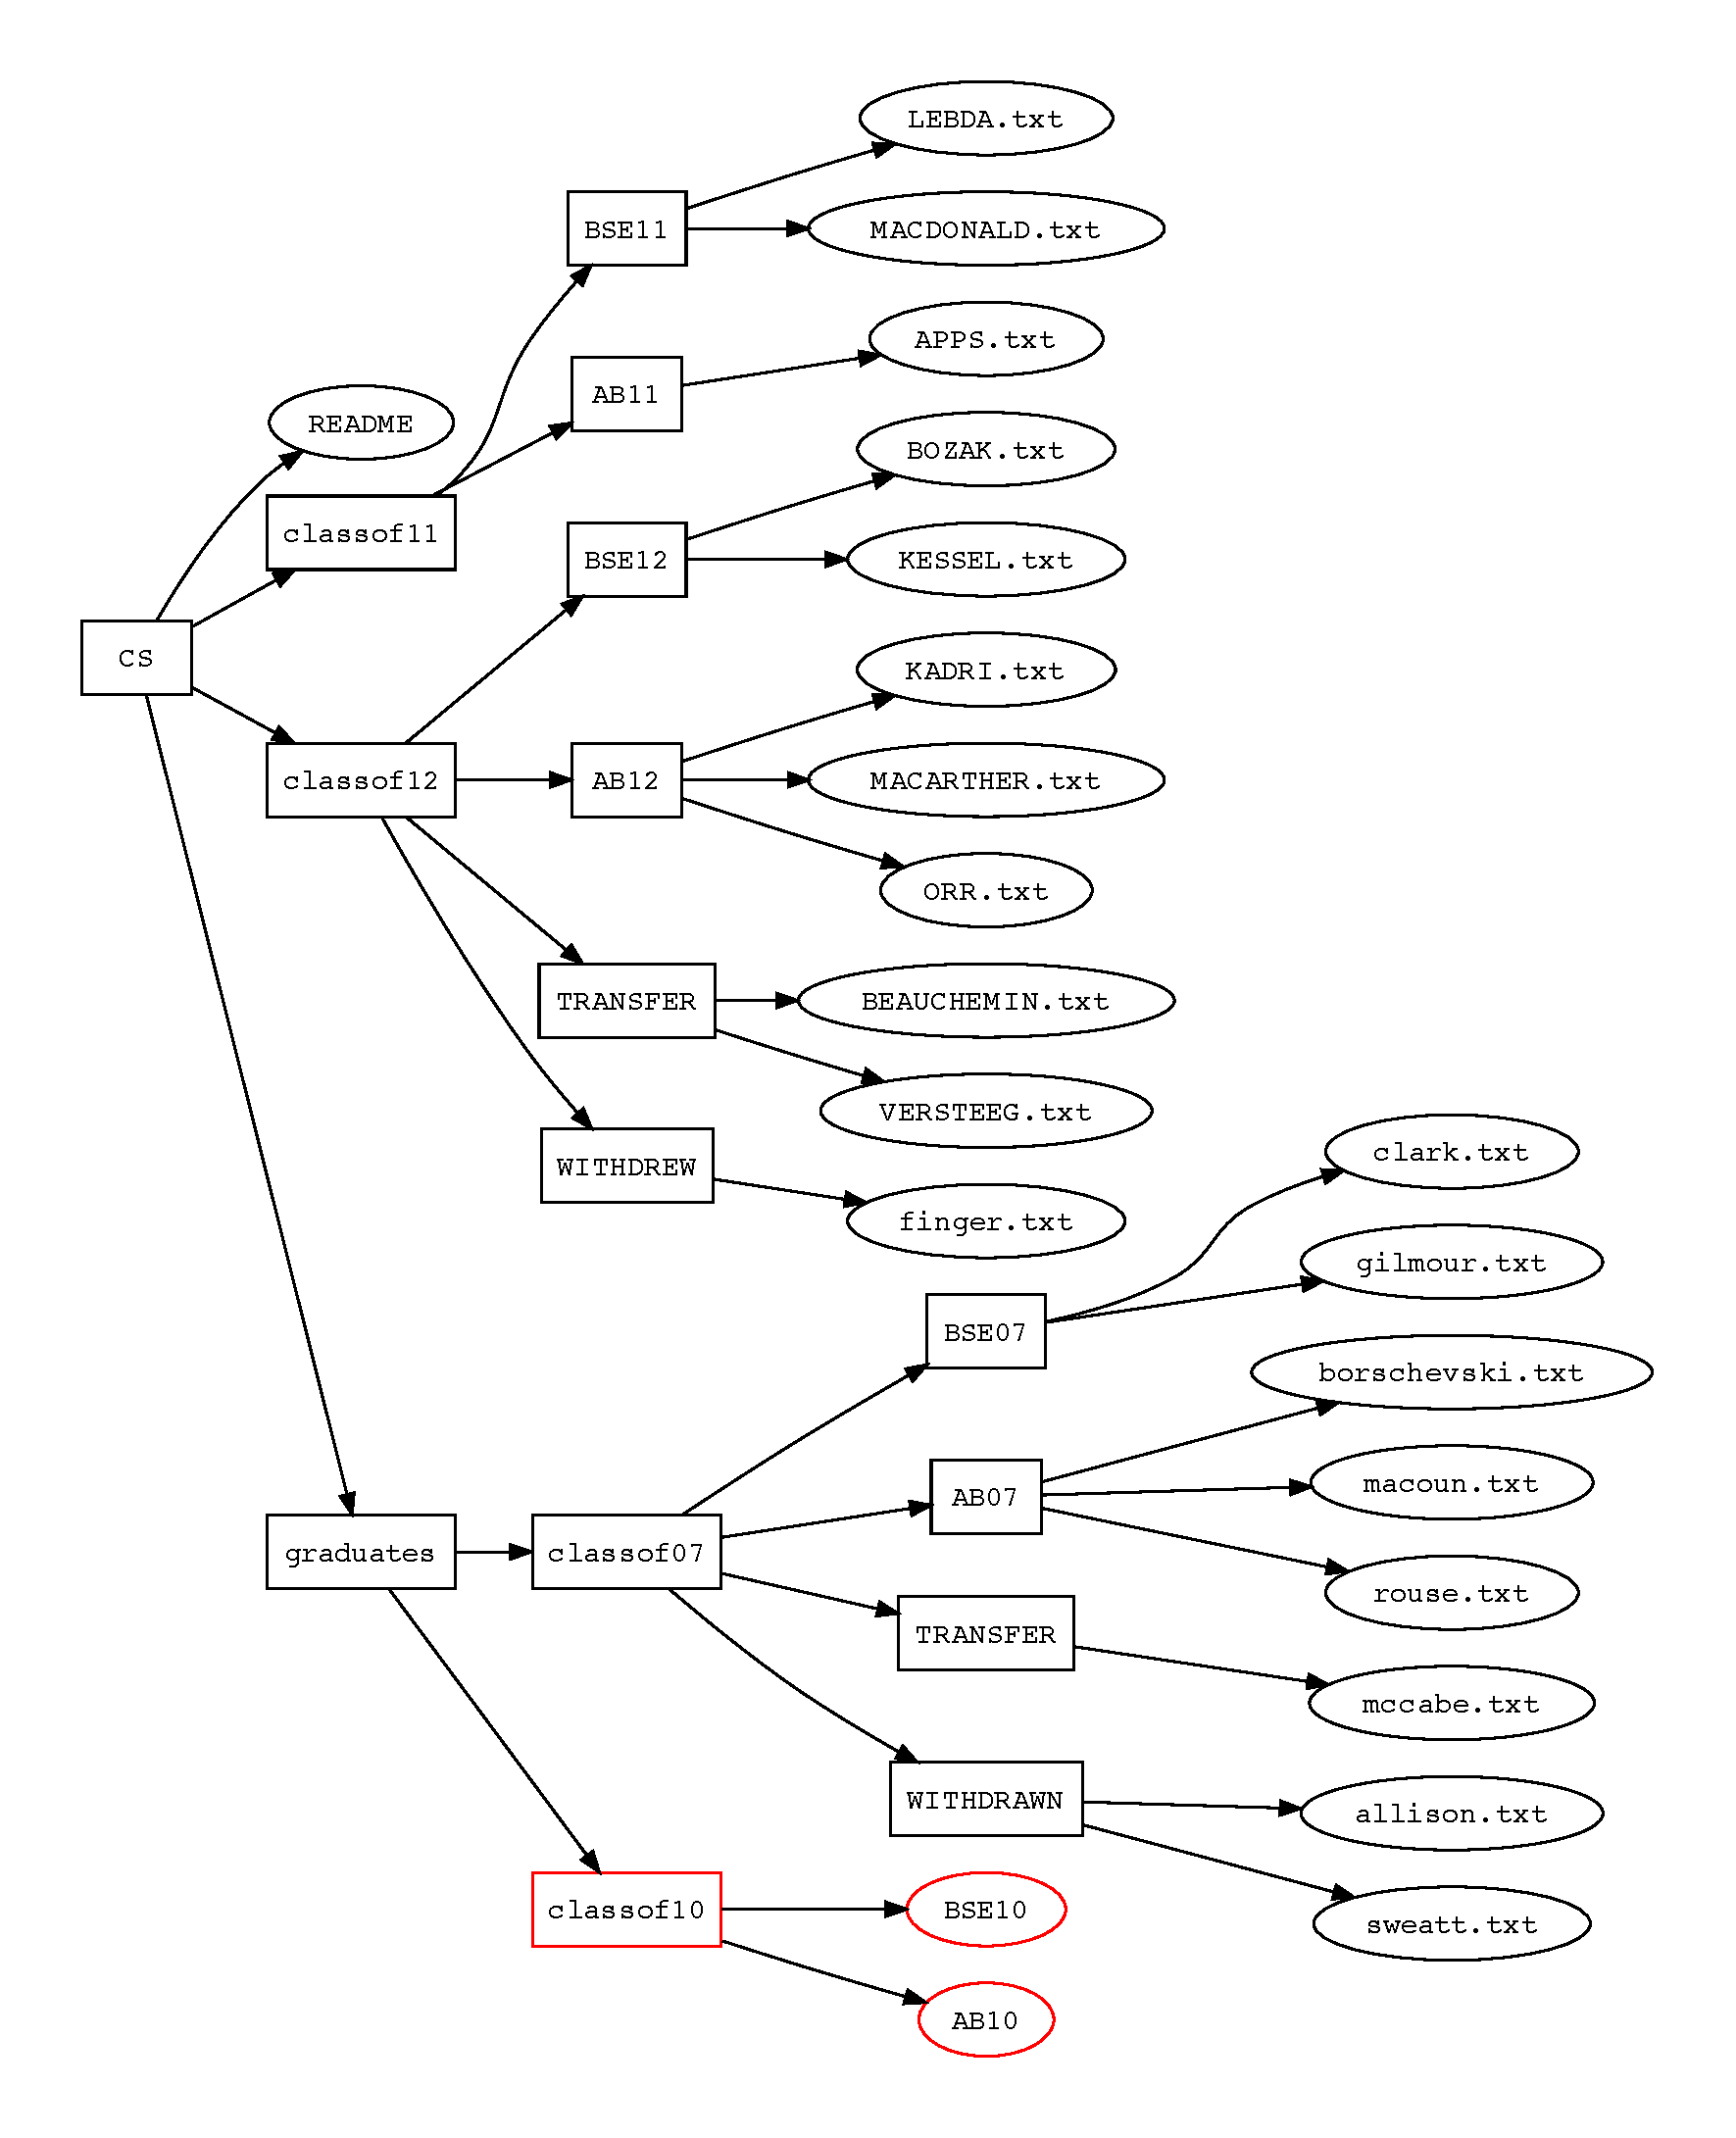
\includegraphics{StudentsNew.pdf}}
\vskip -.1in
\caption{Anonymized snippet of Princeton computer science undergraduate data. Red notes denotes an error---i.e., missing files.}
\reviewer{The lines in the figure appear all to be a single color to
  folks who are red-green color blind.  (And, of course, the
  distinction must be lost in the printed proceedings.)  How about
  different widths instead of different colors?  }
\label{fig:student-pic}
\end{figure}

In this section, we present two example \filestores{}.
We use these examples to motivate and explain
the design of \forest{}.

The first \filestore{} contains information about students in
Princeton's undergraduate computer science program.   
The faculty use the information in the \filestore{}
to decide on undergraduate awards and to track grading trends.
%It was created in approximately 1990 and has been in use ever since.
\reviewer{"as it evolved over time, there have been changes to its format" ->
"its format changed over time"}
%
As it evolved over time, there have been changes to its
format---something that is typical for ad hoc \filestores{}!
Naturally, any description needs to cope with the variations
introduced as formats evolve.
 
Figure~\ref{fig:student-pic} shows a snippet
of the (anonymized) student \filestore{} designed to
illustrate its structure.  At the top level, there are
three directories: 
\cd{classof11} (seniors),
\cd{classof12} (juniors)
and 
\cd{graduates} (students who have graduated).
There is also a \cd{README} file containing a collection of notes.
Inside \cd{graduates}, there is set of directories named 
\cd{classofYY} where \cd{YY} dates back to 92.  Inside each \cd{classofYY} 
directory, there are at least the 
two degree subdirectories \cd{ABYY} and \cd{BSEYY} as
the computer science department gives out both Arts and Science
and Engineering degrees.  Optionally, there are also subdirectories for
students who withdrew from Princeton or transferred to another program. 
Within any degree subdirectory, there is one text file
per student that records the courses taken and the corresponding grades.
%Figure~\ref{fig:student-file-example} shows a fragment
%of a typical student record file.    
%Note that such files can easily be described by a
%data-description language like \pads{}~\cite{fisher+:pads}.
Each degree directory may also contain a 
template file named \cd{sss.txt} or \cd{sxx.txt} for creating
new students.


%% \begin{figure}
%% % Note: Kessel has poor grades in COS but excels in HOC and 
%% % is taking a grad course in GOL(s).  :-)
%% \begin{code}
%% KESSEL, PHIL	   BSE   '11
%% - - - - - - - - - - - - - - - - - - -
%% Type    Yr  Course     Grade
%%          1             A+ to F
%% d        2             P  (  Pass )
%% t  D  p  3             INC
%% o  .  .  4  Dept  xxx  N  (Not Avail)
%% - - - - - - - - - - - - - - - - - - -
%% d  .  .  1  COS   101  C
%% o  .  .  1  HOC   101  A
%% o  .  .  1  GOL   599  A+
%% ...
%% \end{code}
%% \caption{Initial portion of student record file {\tt KESSEL.txt}.}
%% \label{fig:student-file-example}
%% \end{figure}

The second \filestore{} contains log files for 
CoralCDN~\cite{freedman+:coral,freedman:coral-experience}. To
monitor the performance and security of the system, the hosts
participating in CoralCDN periodically send usage statistics back to
a central server. These statistics are collected in a \filestore{}
%similar to the one depicted in Figure~\ref{fig:coral-pic}.
with a top-level directory named \cd{dat}. 
This directory contains a set of subdirectories, 
one for each host, and each of those directories contain
another set of directories, labeled by date and time.
Finally, each of the
date/time directories contain one or more compressed log files. For the
purposes of this example, we will focus on the \cd{coralwebsrv.log.gz}
log file, which contains detailed information about the web requests
made on the host during the preceding time period.  
In addition to exploring this primary \filestore{},
we also explore a secondary, derived \filestore{}. 
This secondary store, named
\cd{stats}, contains files  
that store statistics
generated by \forest{}/Haskell scripts that analyze and
summarize the raw CoralCDN server data.  These system-wide summaries are
representative of the statistics reported by
Freedman~\cite{freedman:coral-experience}.

%\reminder{We should check with Mike that including this information (machine
%  names, dates) is okay. Also, we will probably need to make
%  the graph smaller by eliding some nodes.}

% \begin{figure}
% \vskip -.25in
% \hskip -.15in\scalebox{.31}{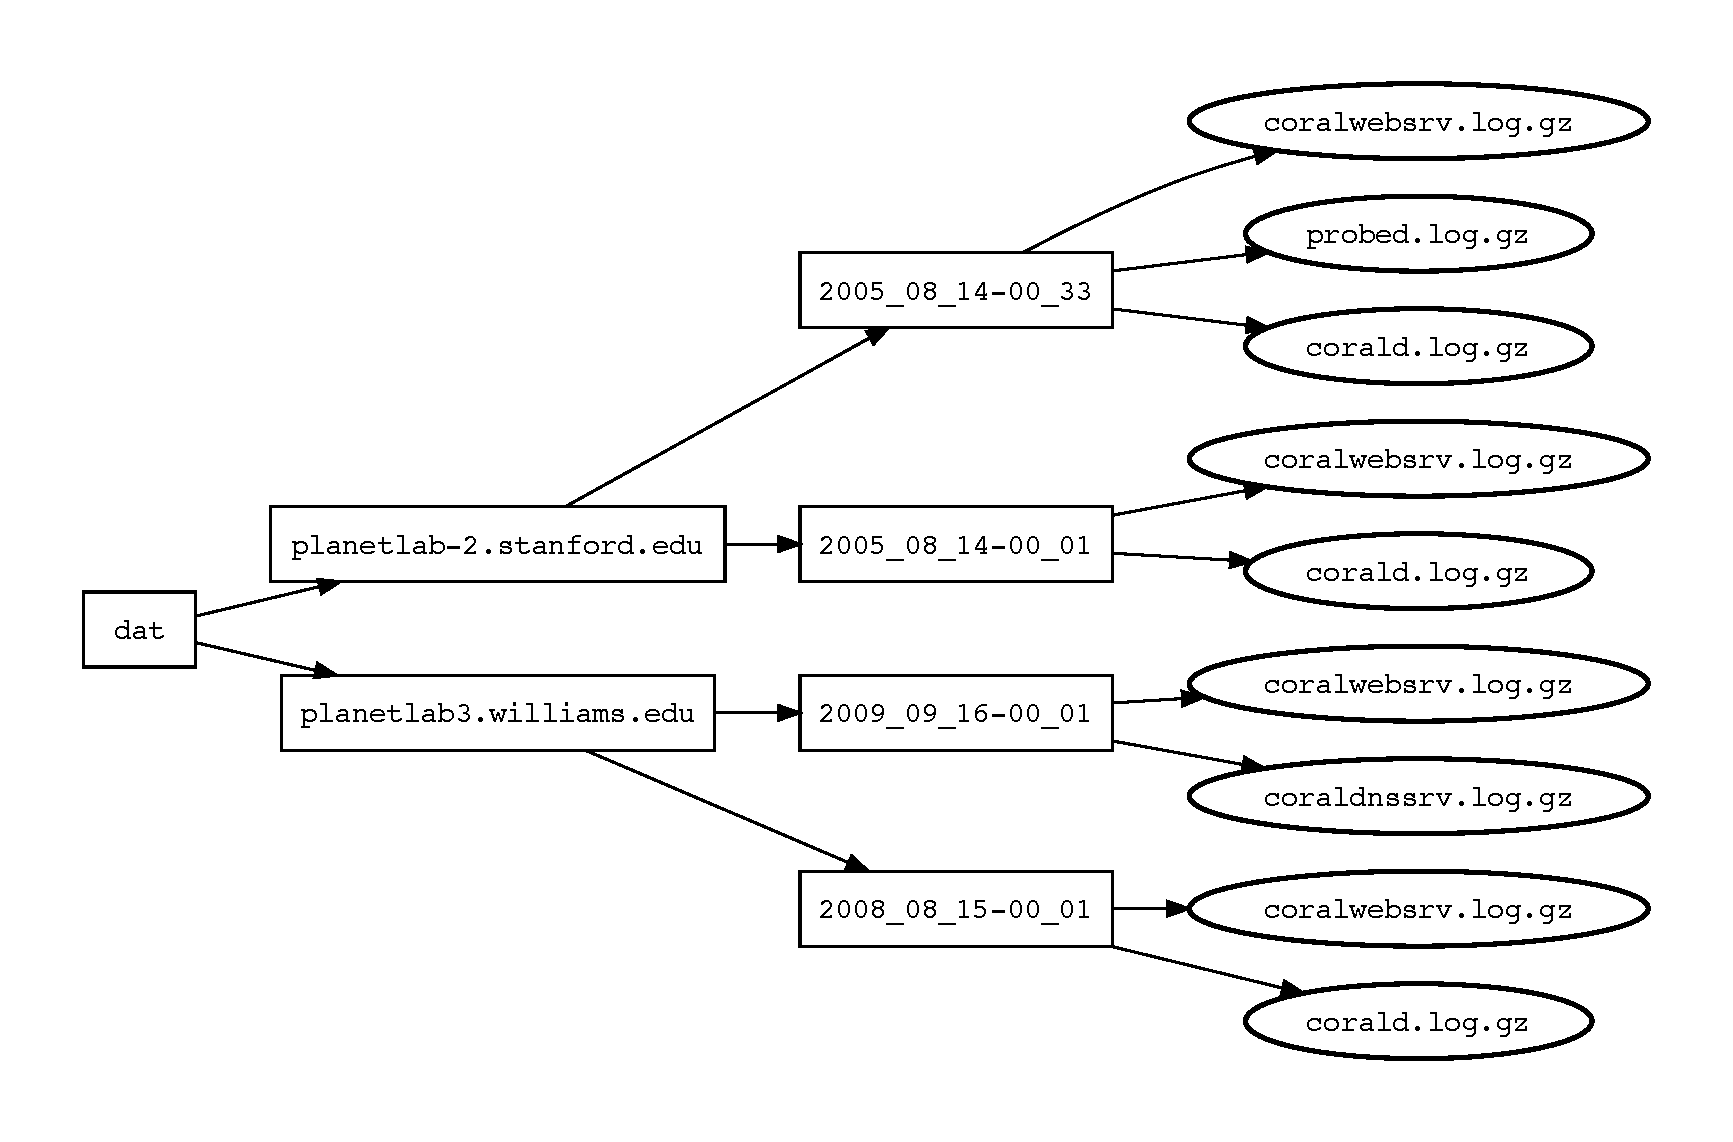
\includegraphics{coral-structure.pdf}}
% \vskip -.1in
% %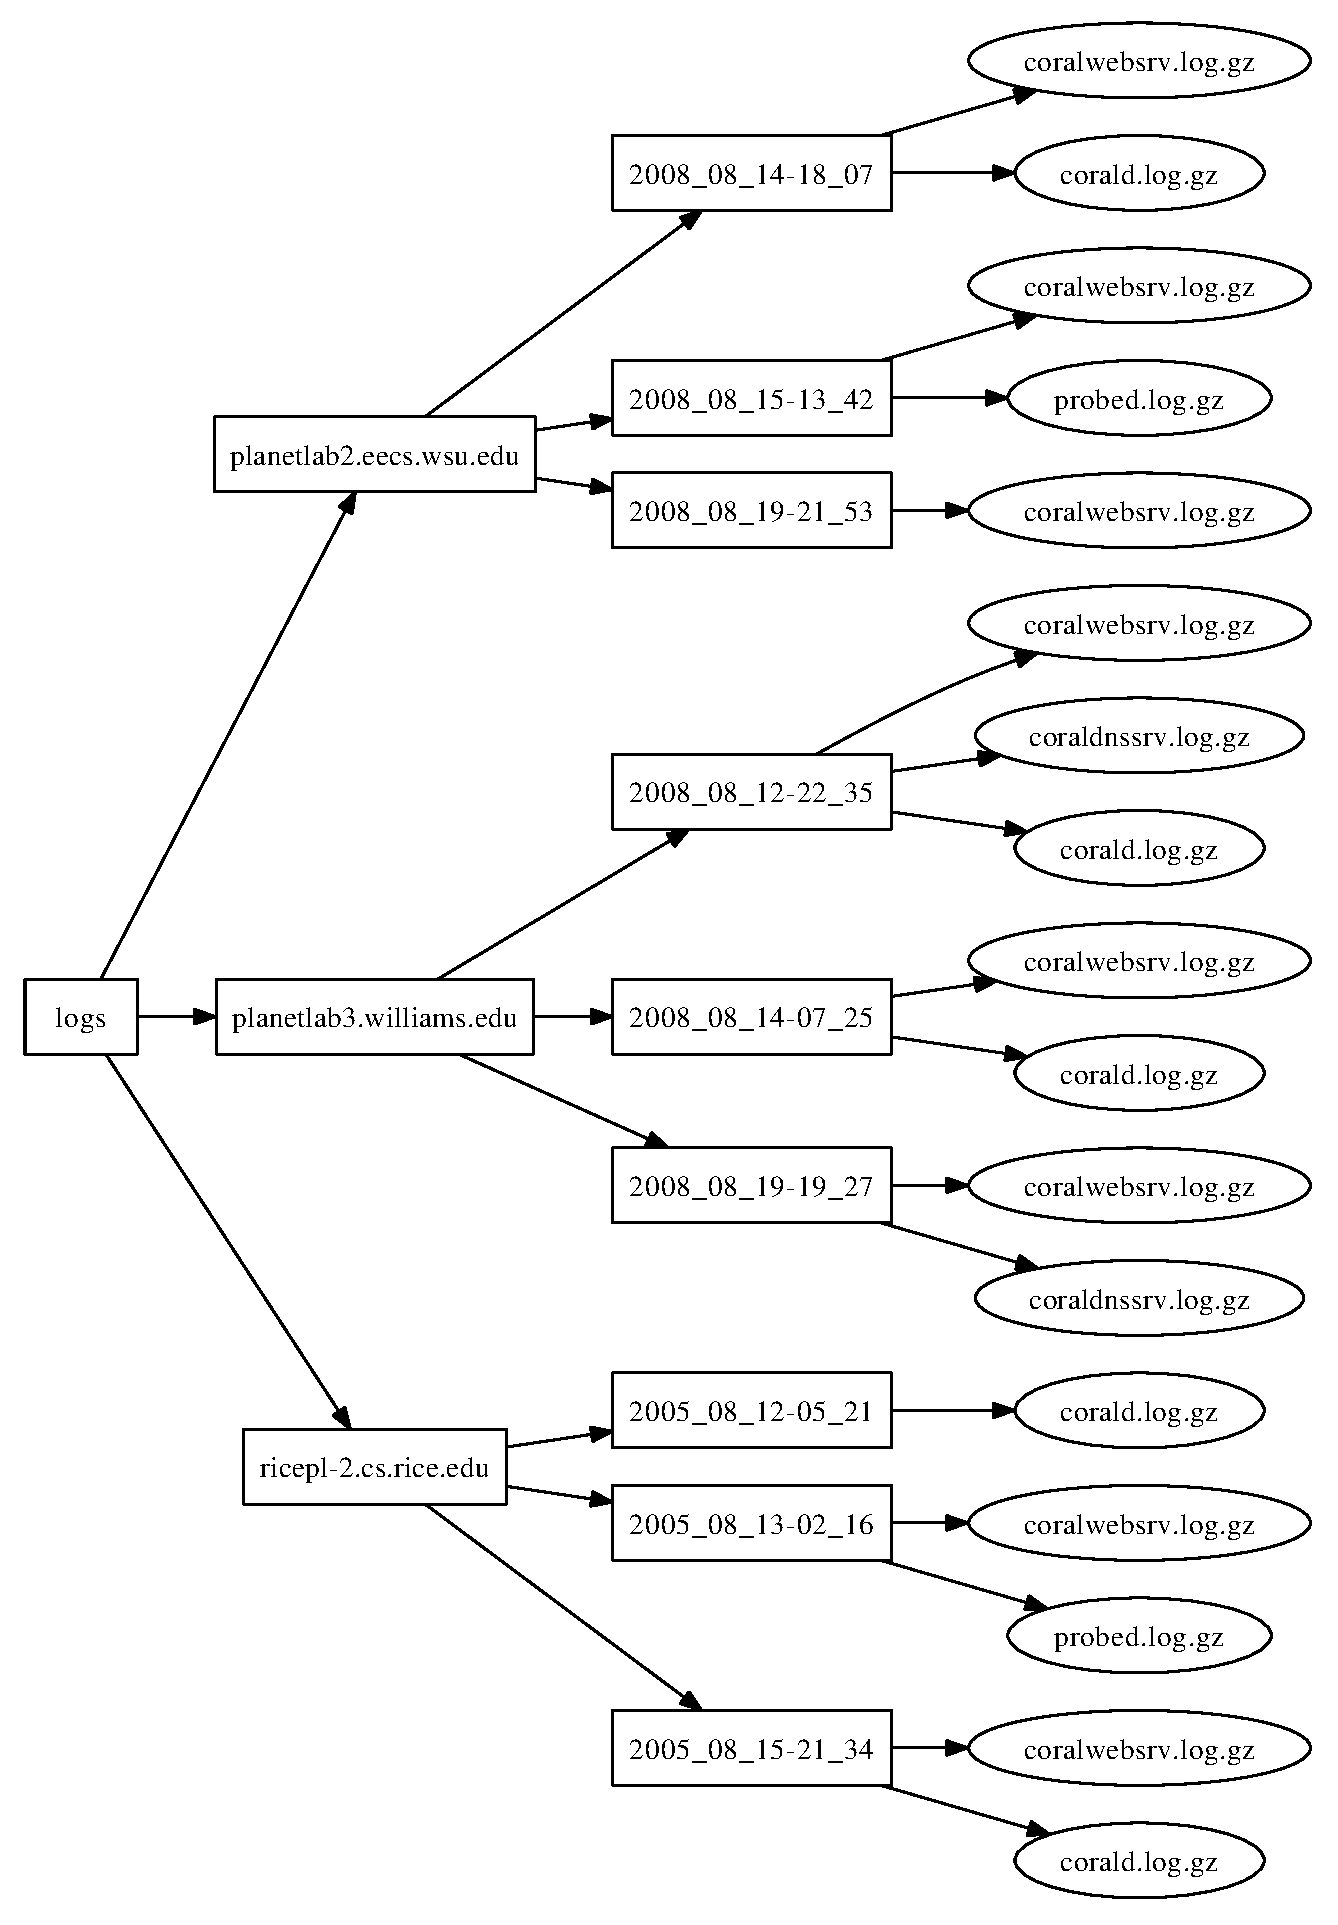
\epsfig{file=coral-structure.eps, width=0.9\columnwidth}
% \caption{Coral system log data.}
% \label{fig:coral-pic}
% \end{figure}

